\documentclass[conference,compsoc]{IEEEtran}

\ifCLASSOPTIONcompsoc
  \usepackage[nocompress]{cite}
\else
  \usepackage{cite}
\fi

\usepackage{amsmath,amssymb}
\usepackage{graphicx}
\usepackage{booktabs}
\usepackage{braket}
\usepackage{xcolor}
\usepackage{enumitem}
\usepackage{multirow}
\setlist{nosep}

\hyphenation{Physio-Net cross-attention multi-basis}

\newcommand{\TODO}[1]{\textcolor{red}{\textbf{[TODO: #1]}}}

\begin{document}

% NOTE: if ISSC requires the paper title to match the submitted abstract verbatim,
% revert to "Quantum-Enhanced Machine Learning Pipeline for Biomedical Image
% Analysis and Diagnostic Applications". The body below is consistent with either.
\title{Quantum-Enhanced Machine Learning for Biomedical Diagnostics:\\An Image-to-ECG Transfer Study on PhysioNet 2017}

\author{\IEEEauthorblockN{Sogodam Atadana\IEEEauthorrefmark{1}, Özlem Karabiber Cura\IEEEauthorrefmark{2}}
\IEEEauthorblockA{%
\IEEEauthorrefmark{1}İzmir Katip Çelebi University, Biomedical Engineering Department, atadanas@gmail.com\\
\IEEEauthorrefmark{2}İzmir Katip Çelebi University, Biomedical Engineering Department, ozlem.karabiber@ikcu.edu.tr
}}

\maketitle

% ==================================================================
\begin{abstract}
A 3-qubit channel-entangled Quantum Probability Image Encoding (QPIE) pipeline that captures label-relevant colour structure on RGB medical images has been reported in companion work. We test whether that image-domain encoding transfers to a clinical time-series task: single-lead electrocardiogram (ECG) arrhythmia classification on the PhysioNet/CinC 2017 AF Challenge. The three colour channels are replaced by three signals manufactured from the ECG itself --- bandpassed amplitude, first difference, and the Hilbert envelope of a \texttt{db4} wavelet-detail band. Six encoding schemes (Sep, CRyE, GBE, CSE, PA-CSE, CP-2L) map each $\sim$0.83\,s window to a 3-qubit state, and Z$+$X$+$Y multi-basis measurement yields 24 features per window. We evaluate three classification heads over five seeds --- an aggregated MLP, a per-window 1D CNN, and QMBC-Net, a cross-attention head built around the (Z, X, Y) measurement structure --- against the published challenge baselines and against a same-representation ROCKET baseline on the raw three channels.
The strongest configuration, a 1D CNN on the per-window features, reaches macro-F1 0.670 on the official N/A/O metric, 16 points below the 0.83 challenge state of the art and 5 points below ROCKET on the identical three channels. Three results hold across every head: the separable encoder matches or beats all entangling schemes, the global Bell entangler is the weakest by 5--7 points, and QMBC-Net trails the plain 1D CNN by ten points. The quantum feature map that helps on RGB MedMNIST does not transfer to single-lead ECG. The advantage on images appears specific to spatial channel correlations that physiological time series lack. We report the negative result, a reusable recipe for porting the encoder to a 1D biosignal, and the regime it delineates.
\end{abstract}

\begin{IEEEkeywords}
Quantum machine learning, electrocardiogram, atrial fibrillation, multi-basis measurement, PhysioNet 2017, biomedical signal classification, transfer, negative result.
\end{IEEEkeywords}

\IEEEpeerreviewmaketitle

% ==================================================================
\section{Introduction}
\label{sec:intro}

Atrial fibrillation (AF) is the most common sustained cardiac arrhythmia and a major cause of stroke. Single-lead wearable ECG has made low-cost screening realistic, and the PhysioNet/CinC 2017 AF Challenge~\cite{clifford2017af} released 8528 short single-lead recordings as a public benchmark. Top entries reach macro-F1 around 0.83 over the three clinical classes (Normal, AF, Other)~\cite{clifford2017af, andreotti2017comparing, goodfellow2018towards}.

Quantum feature extractors are a less explored route, and the evidence on whether they help is thin and domain-specific. In companion work~\cite{atadana2026qpie} we extended QPIE to RGB images by assigning one qubit per colour channel and varying the entangling structure across six schemes; a data-conditional scheme captured label-relevant pixel correlations on PathMNIST. That result is the motivation, not the claim, of this paper. The question here is narrow and falsifiable: does an encoding designed for the spatial channel correlations of RGB images carry over to a 1D physiological signal once the three colour channels are replaced by three engineered signal channels, and does a head built around the structure of multi-basis quantum measurements improve on the standard classical heads?

The answer, on PhysioNet 2017, is no on both counts, and the way it fails is informative. We port the six 3-qubit encoders from~\cite{atadana2026qpie} unchanged, manufacture three signal channels from each recording, and run three classification heads --- an MLP on aggregated features, a 1D CNN on per-window features, and QMBC-Net, a cross-basis-to-temporal attention head designed for multi-basis features. We benchmark against the published challenge baselines and against ROCKET~\cite{dempster2020rocket} on the raw three channels, the same-representation control that isolates what the quantum step adds.

The contributions are three.
\begin{enumerate}
    \item \textbf{A 1D adaptation of the channel-entangled QPIE encoder.} A reusable recipe for porting the 3-channel RGB encoder to any 1D biosignal: bandpassed amplitude, first difference, and a band-limited envelope as the three channels.
    \item \textbf{A controlled transfer test on a clinical benchmark.} Six encoders $\times$ three heads $\times$ five seeds on PhysioNet 2017, scored on the official N/A/O macro-F1, against published baselines and a same-representation ROCKET control.
    \item \textbf{A negative, mechanistic result.} The encoding is lossy (16 points below the challenge state of the art, 5 below same-representation ROCKET); entanglement provides no benefit (the separable scheme is best, the global Bell entangler worst); and QMBC-Net underperforms a plain 1D CNN. The pattern is consistent with the image-domain advantage being specific to spatial channel correlations that single-lead ECG does not contain. A time-delay re-alignment of the encoder input, motivated by this diagnosis, changes which scheme wins but does not recover accuracy, which isolates the fixed encoding --- not the entanglement structure --- as the bottleneck.
\end{enumerate}

Section~\ref{sec:background} reviews the benchmark and quantum encodings. Section~\ref{sec:method} describes the 1D channel construction, the six encoders, and the three heads. Section~\ref{sec:experiments} states the protocol. Section~\ref{sec:results} reports the results. Section~\ref{sec:discussion} reads the negative result against the image-domain mechanism.

% ==================================================================
\section{Background and Related Work}
\label{sec:background}

\subsection{ECG arrhythmia classification on PhysioNet 2017}

The 2017 AF Challenge released 8528 single-lead ECG recordings sampled at 300\,Hz, 9 to 60 seconds long, labelled Normal (N), AF (A), Other (O), or Noise ($\sim$). The official metric is macro-F1 over N/A/O. Class balance is roughly 60/9/28/3 percent, so AF and the heterogeneous Other class dominate the macro average.

The challenge winner used hand-crafted heart-rate-variability and morphology features fed to a gradient-boosted tree, reaching macro-F1 0.83~\cite{clifford2017af}. Andreotti et al.\ compared feature-engineered and convolutional entries and reported 0.79--0.83~\cite{andreotti2017comparing}; Goodfellow et al.\ trained a multi-scale CNN~\cite{goodfellow2018towards}. Hannun et al.\ reached F1 0.83 over 12 rhythm classes on a different and larger single-lead dataset~\cite{hannun2019cardiologist}, reported here only for context.

\subsection{Quantum image and signal encodings}

Quantum image representations include FRQI~\cite{le2011flexible}, NEQR~\cite{zhang2013neqr}, MCQI~\cite{sun2011multi}, and QPIE~\cite{yao2017quantum}; none target temporal signals directly. Adaptations to time series have used amplitude encoding of the signal or angle encoding of windowed features~\cite{kyriienko2022unsupervised}. In~\cite{atadana2026qpie} the six 3-qubit encoders below were validated on MedMNIST, where multi-basis measurement and statistical aggregation produced a 492-dimensional feature vector competitive with a small CNN. This paper reuses those encoders and the measurement pipeline without modification, which is what makes the transfer question clean.

\subsection{Attention over quantum measurements}

Standard heads treat quantum-feature outputs as plain vectors and discard the (Z, X, Y) basis structure. QMBC-Net attends across measurement bases as named tokens before attending across time; the closest prior design is multi-modal cross-attention~\cite{vaswani2017attention}. We include it as a candidate head to test, not as an established method.

% ==================================================================
\section{Method}
\label{sec:method}

\subsection{From single-lead ECG to three signal channels}

A recording $x[n]$ is bandpass-filtered to 0.5--40\,Hz and centre-cropped or zero-padded to 30\,s ($N = 9000$ at 300\,Hz). For each recording we form three channels:
\begin{align}
    c_1[n] &= x_\text{bp}[n] && \text{(bandpassed amplitude)} \\
    c_2[n] &= x_\text{bp}[n] - x_\text{bp}[n-1] && \text{(first difference)} \\
    c_3[n] &= |\mathcal{H}\{w_{d}[n]\}| && \text{(wavelet-detail envelope)}
\end{align}
where $w_{d}$ is the level-2 detail of a five-level \texttt{db4} wavelet decomposition of the bandpassed signal (nominal 37.5--75\,Hz octave, with content limited by the 0.5--40\,Hz passband) and $\mathcal{H}$ is the Hilbert transform. Each channel is robust-scaled per-recording with the q5/q95 mapping from~\cite{atadana2026qpie} into $[0,1]$. Figure~\ref{fig:channels} shows the three channels on a sample recording.

\begin{figure}[t]
\centering
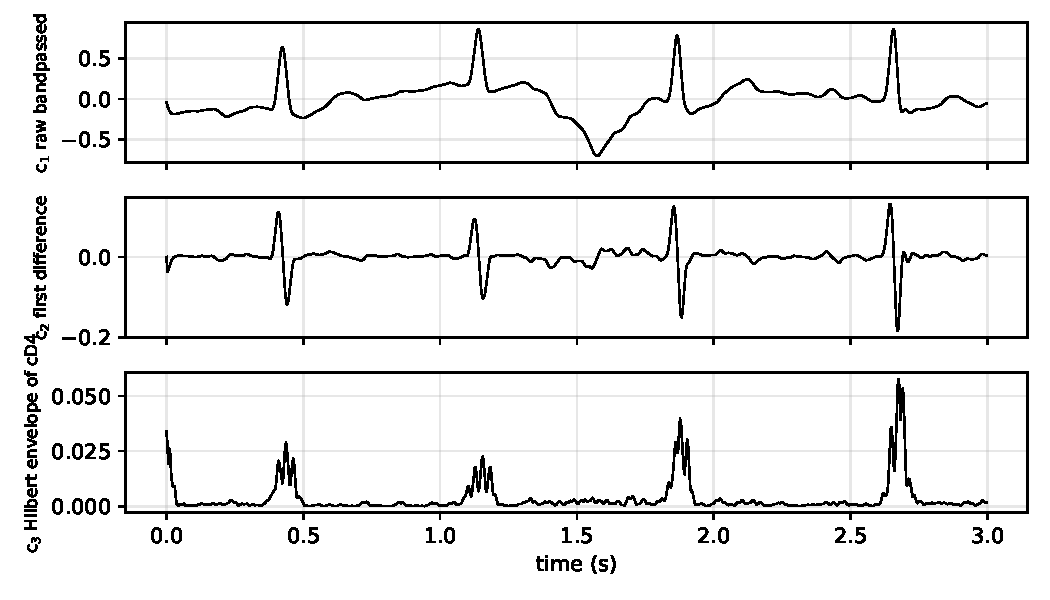
\includegraphics[width=\columnwidth]{figures/fig_three_channels.pdf}
\caption{The three signal channels built from one ECG recording: bandpassed amplitude, first difference, and the \texttt{db4} wavelet-detail envelope. These replace the three colour channels of the RGB encoder.}
\label{fig:channels}
\end{figure}

\subsection{Per-window 3-qubit encoding}

The signal is split into windows of 250 samples ($\sim$0.83\,s, near one cardiac cycle) with stride 125, giving $W = 71$ windows. We reuse all six encoders from~\cite{atadana2026qpie}: Sep (separable, per-channel angle encoding only), CRyE and GBE (controlled-$R_y$ and global Bell entanglers), CSE and PA-CSE (data-conditional schemes whose entangling angles depend on pairwise channel correlations), and CP-2L (a two-layer encode--entangle circuit). Each takes a 3-channel sample $(\bar c_1,\bar c_2,\bar c_3)\in[0,1]^3$ and returns a 3-qubit amplitude vector; shared angle encoding $\theta_c=\pi\bar c_c$; the schemes differ only in the entangling gates. We project each per-sample state onto Z, X, and Y (24 features), and aggregate over the window. The per-window mean gives a $(W\times 24)$ sequence; full per-sample aggregation gives a 492-dimensional recording vector ($9{\times}24$ statistics $+\binom{24}{2}$ correlations).

\subsection{Three classification heads}

\textbf{Phase-1A: aggregated MLP.} The 492-dimensional recording vector through the MedMNIST MLP head from~\cite{atadana2026qpie}: $512\to256\to128\to4$ with BatchNorm, ReLU, Dropout 0.3.

\textbf{Phase-1B: 1D CNN over windows.} The $(W\times 24)$ per-window sequence through a three-block 1D CNN with dilations $\{1,2,4\}$, adaptive average pooling, and a linear classifier. The aggregation step is removed; the CNN sees temporal order.

\textbf{Phase-2: QMBC-Net.} Per window, the 24 features split into three basis tokens of 8 (Z, X, Y), embed to dimension 64, and pass through one cross-basis multi-head attention layer; a learned per-basis gate pools the three tokens to a window vector. Sinusoidal positional encoding over windows precedes two layers of temporal self-attention; a CLS token feeds a linear classifier. The design exposes which basis and which windows the model relies on.

% ==================================================================
\section{Experimental Setup}
\label{sec:experiments}

PhysioNet/CinC 2017 AF Challenge~\cite{clifford2017af}, 8528 recordings, 4 classes, loaded via \texttt{wfdb} with the rescored REFERENCE-v3 labels. Stratified 60/20/20 split across N/A/O/$\sim$. All heads use AdamW (lr $10^{-3}$, weight decay $10^{-4}$), cosine annealing, square-root class-weighted cross-entropy, batch 256, up to 100 epochs, early stopping on validation macro-F1 with patience 20; five seeds; Apple M4, MPS backend.

The primary metric is macro-F1 over N/A/O (Noise excluded), the official challenge metric; secondary metrics are macro AUC (one-vs-rest) and balanced accuracy. We compare against the published baselines (Table~\ref{tab:sota}) and against multivariate ROCKET~\cite{dempster2020rocket} on the raw three channels with the identical split and metric --- the same-representation control that separates the encoding's contribution from the representation's.

% ==================================================================
\section{Results}
\label{sec:results}

The headline is in Table~\ref{tab:sota}: the best quantum configuration reaches macro-F1 0.670, well below both the published baselines and same-representation ROCKET. Within that ceiling, three patterns recur across the three heads.

\subsection{Across heads: the separable scheme is not beaten}

Tables~\ref{tab:phase1a}--\ref{tab:phase2} report all six schemes through each head over five seeds; Fig.~\ref{fig:phase1} plots the two Phase-1 heads. No entangling scheme beats the separable baseline (Sep) on any head. On the strongest head (1D CNN) Sep (0.669) and the data-conditional PA-CSE (0.670) are tied best, while the global Bell entangler GBE is worst at 0.598 --- a 7-point entanglement penalty. In QMBC-Net the ordering is the same, with GBE the weakest scheme (9 points below Sep); in the aggregated MLP the six schemes fall within roughly one point of each other, so that head is too coarse to separate them. Entanglement, fixed or data-conditional, adds nothing here.

\begin{table}[t]
\caption{Phase-1A --- aggregated MLP, PhysioNet 2017, 5 seeds.}
\label{tab:phase1a}
\centering
\begin{tabular}{lccc}
\toprule
Scheme & macro-F1 & AUC & BAcc \\
\midrule
Sep    & 0.533 $\pm$ 0.012 & 0.801 $\pm$ 0.003 & 0.594 $\pm$ 0.015 \\
CRyE   & 0.521 $\pm$ 0.004 & 0.786 $\pm$ 0.002 & 0.565 $\pm$ 0.008 \\
GBE    & 0.522 $\pm$ 0.006 & 0.799 $\pm$ 0.001 & 0.591 $\pm$ 0.004 \\
CSE    & 0.522 $\pm$ 0.007 & 0.786 $\pm$ 0.003 & 0.568 $\pm$ 0.008 \\
PA-CSE & 0.526 $\pm$ 0.006 & 0.792 $\pm$ 0.005 & 0.580 $\pm$ 0.009 \\
CP-2L  & 0.526 $\pm$ 0.006 & 0.799 $\pm$ 0.002 & 0.593 $\pm$ 0.005 \\
\bottomrule
\end{tabular}
\end{table}

\begin{table}[t]
\caption{Phase-1B --- 1D CNN over windows, PhysioNet 2017, 5 seeds. Best head.}
\label{tab:phase1b}
\centering
\begin{tabular}{lccc}
\toprule
Scheme & macro-F1 & AUC & BAcc \\
\midrule
Sep    & 0.669 $\pm$ 0.005 & 0.891 $\pm$ 0.001 & 0.688 $\pm$ 0.009 \\
CRyE   & 0.642 $\pm$ 0.012 & 0.878 $\pm$ 0.005 & 0.662 $\pm$ 0.008 \\
GBE    & 0.598 $\pm$ 0.006 & 0.855 $\pm$ 0.003 & 0.614 $\pm$ 0.018 \\
CSE    & 0.621 $\pm$ 0.009 & 0.872 $\pm$ 0.002 & 0.651 $\pm$ 0.007 \\
PA-CSE & \textbf{0.670} $\pm$ 0.004 & 0.887 $\pm$ 0.001 & 0.682 $\pm$ 0.007 \\
CP-2L  & 0.659 $\pm$ 0.013 & 0.886 $\pm$ 0.003 & 0.665 $\pm$ 0.013 \\
\bottomrule
\end{tabular}
\end{table}

\subsection{Aggregation discards temporal order}

The MLP on aggregated features tops out at 0.533 (Sep), 14 points below the same encoder through the 1D CNN (0.669). Pooling per-sample statistics over the recording removes the temporal structure that distinguishes rhythms, and the CNN recovers it. This mirrors the pooled-versus-CNN gap reported for the same encoders on gesture time series, and locates the useful signal in window order rather than in the per-window statistics.

\subsection{QMBC-Net does not beat a plain CNN}

QMBC-Net was included to test whether a head built around the measurement bases helps. It does not (Table~\ref{tab:phase2}). Its best scheme reaches 0.562 (Sep), ten points below the 1D CNN. The basis-token attention adds parameters and structure without accuracy; the per-basis gates do not concentrate on any single projection axis. The architectural claim is not supported, and we do not advance QMBC-Net as a contribution beyond this negative finding.

\begin{table}[t]
\caption{Phase-2 --- QMBC-Net, PhysioNet 2017, 5 seeds.}
\label{tab:phase2}
\centering
\begin{tabular}{lccc}
\toprule
Scheme & macro-F1 & AUC & BAcc \\
\midrule
Sep    & 0.562 $\pm$ 0.005 & 0.829 $\pm$ 0.001 & 0.584 $\pm$ 0.007 \\
CRyE   & 0.511 $\pm$ 0.011 & 0.800 $\pm$ 0.002 & 0.536 $\pm$ 0.001 \\
GBE    & 0.473 $\pm$ 0.009 & 0.767 $\pm$ 0.004 & 0.516 $\pm$ 0.016 \\
CSE    & 0.532 $\pm$ 0.011 & 0.815 $\pm$ 0.007 & 0.561 $\pm$ 0.023 \\
PA-CSE & 0.547 $\pm$ 0.009 & 0.822 $\pm$ 0.005 & 0.569 $\pm$ 0.008 \\
CP-2L  & 0.534 $\pm$ 0.012 & 0.817 $\pm$ 0.003 & 0.567 $\pm$ 0.017 \\
\bottomrule
\end{tabular}
\end{table}

\begin{figure}[t]
\centering
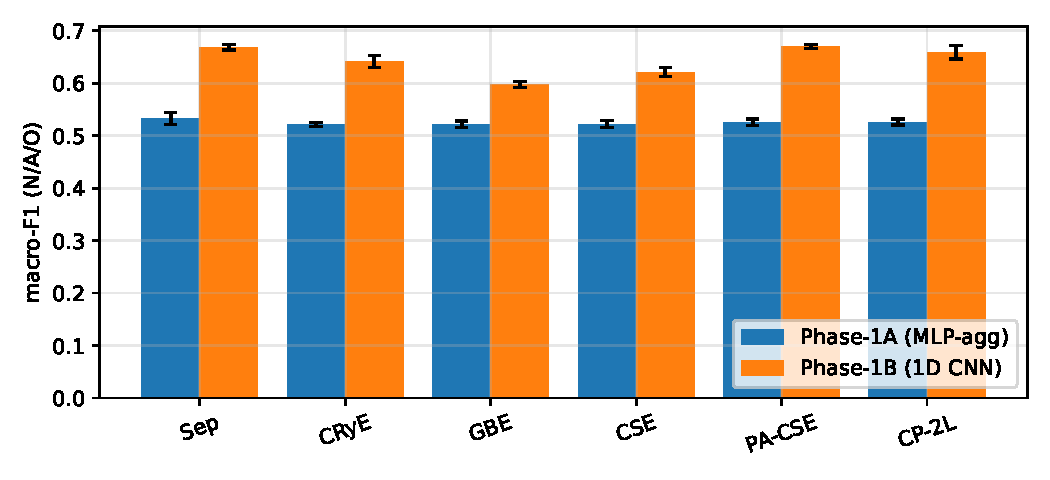
\includegraphics[width=\columnwidth]{figures/fig_phase1_results.pdf}
\caption{Macro-F1 (N/A/O) per scheme for the aggregated MLP (Phase-1A) and the 1D CNN (Phase-1B), 5 seeds. The CNN lifts every scheme by recovering temporal order; the separable Sep is best or tied, and the global Bell entangler GBE is consistently weakest.}
\label{fig:phase1}
\end{figure}

\subsection{Same-representation baseline and the published state of the art}

Multivariate ROCKET on the raw three channels reaches macro-F1 $0.719 \pm 0.007$ (5 seeds), above the best quantum configuration by 5 points on the identical representation and split. Per-class F1 for ROCKET is 0.85 (N), 0.70 (AF), 0.61 (Other); the heterogeneous Other class is the hardest for every method. A fast random-convolution baseline on the same channels is therefore stronger than the quantum encoding, and all of these sit below the 0.83 challenge state of the art, which used richer hand-crafted morphology and rhythm features. The encoding does not reach competitive accuracy and loses to a strong classical baseline on equal footing; the contribution of this work is the transfer behaviour and the boundary it marks, not accuracy.

\begin{table}[t]
\caption{PhysioNet 2017 macro-F1 (N/A/O) --- published baselines, a same-representation control, and ours.}
\label{tab:sota}
\centering
\begin{tabular}{llc}
\toprule
System & Backbone & macro-F1 \\
\midrule
Clifford 2017~\cite{clifford2017af}          & GBT + features      & 0.83 \\
Andreotti 2017~\cite{andreotti2017comparing} & CNN                 & 0.79--0.83 \\
Goodfellow 2018~\cite{goodfellow2018towards} & multi-scale CNN     & 0.83 \\
Hannun 2019~\cite{hannun2019cardiologist}$^\dagger$ & 34-layer 1D ResNet & 0.83 \\
\midrule
ROCKET (raw 3-ch, this work)$^\S$ & random conv.        & 0.719 \\
Ours, Phase-1A (Sep)             & MLP-agg             & 0.533 \\
Ours, Phase-2 (Sep)              & QMBC-Net            & 0.562 \\
Ours, Phase-1B (PA-CSE)          & 1D CNN              & \textbf{0.670} \\
\bottomrule
\end{tabular}\\[2pt]
\footnotesize $^\dagger$ Different dataset (12 rhythm classes); context only.
$^\S$ Multivariate ROCKET~\cite{dempster2020rocket} on the raw three channels, identical split and metric (this work).
\end{table}

% ==================================================================
\section{Discussion}
\label{sec:discussion}

\subsection{Why the transfer fails}

On RGB MedMNIST the data-conditional schemes helped because adjacent colour channels carry label-relevant correlations that the entangling angles can encode~\cite{atadana2026qpie}. Single-lead ECG has no analogue. The three channels here are deterministic transforms of one signal (amplitude, derivative, envelope), so their cross-channel correlations are fixed by construction and carry little class information. The encoder's representational budget --- which on images is spent on inter-channel structure --- has little to act on, and the entangling schemes collapse toward the separable baseline or below it. The global Bell entangler, which forces correlation regardless of the data, is consistently the worst head: imposed entanglement disrupts rather than helps. This is the image result read in reverse, and it bounds where the encoding is useful: domains with genuine, label-relevant channel correlation, not arbitrary multichannel signals.

\subsection{The encoding is lossy}

The same-representation ROCKET baseline is the sharper statement. Given the identical three channels, a random-convolution model extracts 5 more points of macro-F1 than the best quantum pipeline. The quantum feature map discards label-relevant structure that a cheap classical transform keeps. Aggregation compounds the loss --- the MLP path drops a further 14 points by pooling away temporal order --- which is why the 1D CNN, the head that preserves window order, is the only one to approach ROCKET.

\subsection{Re-aligning the input geometry does not rescue it}

If the entanglement conditions on the wrong correlation axis, the natural correction is to feed the three qubits a time-delay (Takens) embedding $x[t], x[t-\tau], x[t-2\tau]$ of the signal rather than the three derived channels. The data-conditional schemes then condition on lag-$\tau$ autocorrelation, which on ECG tracks rhythm regularity --- the structure that separates AF from sinus rhythm. We tested this on a 3000-recording stratified subset at two lag scales. Morphology-scale lags ($\tau\approx0.1$\,s) left the ordering unchanged: the separable scheme stayed best. At rhythm scale ($\tau\approx0.5$\,s, multi-beat windows) the data-conditional PA-CSE became the only entangling scheme in any of our experiments to exceed the separable baseline (0.47 vs.\ 0.43 macro-F1, three seeds), which is consistent with the mechanism above. The re-alignment did not improve absolute accuracy, however: every delay configuration trailed the simpler channel pipeline. Re-pointing the encoding's conditioning axis changes which scheme wins but not the ceiling. The limitation therefore sits in the fixed encoding itself, not in the entanglement structure or the input geometry, and a trainable, data-driven encoding rather than a fixed circuit is the route a future study should take.

\subsection{What the negative result is good for}

The 1D channel recipe is reusable and the protocol is a template for testing any image-domain quantum encoder on a biosignal before assuming transfer. The ablation also behaves as a diagnostic: the separable-versus-entangled gap measures whether a dataset's channel correlations are label-relevant, and on ECG it reads near zero, consistent with the signal's structure. The honest reading is that the image-domain advantage is modality-specific, and that single-lead ECG diagnostics are better served by classical convolutional or feature-engineered baselines. Clinically, this is a useful caution: a screening tool built on this encoding would underperform a fast classical baseline on the same signal, so the contribution is to map where quantum encoding can and cannot help as such tools are developed, rather than to deploy it now.

\subsection{Limitations}

Single-lead only; PhysioNet 2017 is four-class with strong imbalance, and the macro average is dominated by AF and Other. The three qubits are classically simulable and we make no quantum-advantage claim. Windows are fixed at 250 samples and the split is recording-level, not patient-stratified. The same-representation control uses ROCKET; a deeper classical baseline on the raw channels would tighten the ceiling but not change the direction of the result.

% ==================================================================
\section{Conclusion}
\label{sec:conclusion}

We tested whether a quantum image-encoding pipeline transfers to single-lead ECG arrhythmia classification. It does not. The best configuration, a 1D CNN on the multi-basis features, reaches macro-F1 0.670 on PhysioNet 2017 --- 16 points below the challenge state of the art and 5 below ROCKET on the identical three channels --- no entangling scheme beats the separable baseline, and a measurement-structured attention head underperforms a plain CNN. The advantage the encoder shows on RGB images depends on label-relevant channel correlations that single-lead ECG lacks. Re-aligning the encoder input to temporal-delay coordinates changes which scheme wins but not the accuracy ceiling, which points to a trainable encoding, rather than a fixed circuit, as the next step. We contribute a reusable 1D-adaptation recipe, a controlled transfer protocol, and a clear delineation of the regime in which this class of quantum encoding helps.

% ==================================================================
\ifCLASSOPTIONcompsoc
  \section*{Acknowledgments}
\else
  \section*{Acknowledgment}
\fi

The authors used a large language model to assist with editing and proofreading of the manuscript text. All experiments, results, analysis, and scientific claims are the authors' own and were verified against the source code and data.

% ==================================================================
\begin{thebibliography}{99}

\bibitem{clifford2017af}
G.~D.~Clifford, C.~Liu, B.~Moody, L.-W.~H.~Lehman, I.~Silva, Q.~Li, A.~E.~Johnson, and R.~G.~Mark,
``{AF} classification from a short single lead {ECG} recording: The {PhysioNet}/Computing in Cardiology Challenge 2017,''
in \emph{Proc. Computing in Cardiology}, vol.~44, 2017, pp.~1--4.

\bibitem{hannun2019cardiologist}
A.~Y.~Hannun, P.~Rajpurkar, M.~Haghpanahi, G.~H.~Tison, C.~Bourn, M.~P.~Turakhia, and A.~Y.~Ng,
``Cardiologist-level arrhythmia detection and classification in ambulatory electrocardiograms using a deep neural network,''
\emph{Nature Medicine}, vol.~25, no.~1, pp.~65--69, 2019.

\bibitem{andreotti2017comparing}
F.~Andreotti, O.~Carr, M.~A.~F.~Pimentel, A.~Mahdi, and M.~De~Vos,
``Comparing feature-based classifiers and convolutional neural networks to detect arrhythmia from short segments of {ECG},''
in \emph{Proc. Computing in Cardiology}, vol.~44, 2017, pp.~1--4.

\bibitem{goodfellow2018towards}
S.~D.~Goodfellow, A.~Goodwin, R.~Greer, P.~C.~Laussen, M.~Mazwi, and D.~Eytan,
``Towards understanding {ECG} rhythm classification using convolutional neural networks and attention mappings,''
in \emph{Proc. Mach. Learn. Healthcare}, 2018.

\bibitem{atadana2026qpie}
S.~Atadana and Ö.~Karabiber Cura,
``When does entanglement help in quantum image encoding? A per-image mechanism test on {MedMNIST},''
in \emph{Proc. IEEE Int. Conf. Quantum Comput. Eng. (QCE)}, 2026, to appear.

\bibitem{yao2017quantum}
X.-W.~Yao, H.~Wang, Z.~Liao, M.-C.~Chen \emph{et al.},
``Quantum image processing and its application to edge detection: Theory and experiment,''
\emph{Phys. Rev. X}, vol.~7, p.~031041, 2017.

\bibitem{le2011flexible}
P.~Q.~Le, F.~Dong, and K.~Hirota,
``A flexible representation of quantum images for polynomial preparation, image compression, and processing operations,''
\emph{Quantum Inf. Process.}, vol.~10, no.~1, pp.~63--84, 2011.

\bibitem{zhang2013neqr}
Y.~Zhang, K.~Lu, Y.~Gao, and M.~Wang,
``{NEQR}: A novel enhanced quantum representation of digital images,''
\emph{Quantum Inf. Process.}, vol.~12, no.~8, pp.~2833--2860, 2013.

\bibitem{sun2011multi}
B.~Sun, A.~M.~Iliyasu, F.~Yan, F.~Dong, and K.~Hirota,
``Multi-channel representation for images on quantum computers using the {RGB}$\alpha$ color space,''
in \emph{Proc. IEEE 7th Int. Symp. Intell. Signal Process.}, 2011, pp.~1--6.

\bibitem{dempster2020rocket}
A.~Dempster, F.~Petitjean, and G.~I.~Webb,
``{ROCKET}: Exceptionally fast and accurate time series classification using random convolutional kernels,''
\emph{Data Min. Knowl. Discov.}, vol.~34, no.~5, pp.~1454--1495, 2020.

\bibitem{kyriienko2022unsupervised}
O.~Kyriienko, A.~E.~Paine, and V.~E.~Elfving,
``Protocols for trainable and differentiable quantum generative modelling,''
\emph{Phys. Rev. Research}, vol.~4, p.~043067, 2022.

\bibitem{vaswani2017attention}
A.~Vaswani \emph{et al.},
``Attention is all you need,''
in \emph{Adv. Neural Inf. Process. Syst.}, vol.~30, 2017.

\end{thebibliography}

\end{document}
